\documentclass{report}
\usepackage[francais ]{babel}
\usepackage[utf8]{inputenc}
\usepackage[T1]{fontenc}
\usepackage{graphicx}
\usepackage{float}
\usepackage{hyperref}
\usepackage{array}
\title{\Huge Guide d'utilisateur \\ \huge Mini Games }

\author{M. \textsc{Friedli}, A. \textsc{Gillioz}, J. \textsc{Guerne}\\
He-Arc Ingénierie\\
2000 Neuchatel}
\date{\today{}}
\begin{document}
\maketitle

\chapter{Installation}
Ce chapitre va présenter les différentes démarches nécessaires à l'installation du
programme client et du programme serveur.
\section{Client}

\subsection{Ordinateur}
Pour installer le programme client sur un ordinateur, il est nécessaire d'avoir, au préalable, installé une version récente de Java.
Une fois fait, le fichier client.jar pourra être lancé par un double clic ou par ligne de commande.

\subsection{Android}
Il faut commencer par transéfer l'apk sur l'appareil Android, ensuite en allant chercher le fichier avec le gestionnaire de fichier de
l'appareil, vous pourrez l'exécuter et il vous indiquera les différentes étapes à valider.

\section{Serveur}
Le serveur peut se lancer uniquement sur un ordinateur. Pour le lancer il est péférable d'exécuter le fichier serveur.jar avec la ligne de commande, le programme n'ayant
pas d'interface graphique.


\chapter{Connexion}
Pour jouer il faut commencer par se connecter à un serveur.
Au lancement du programme vous devrez donc entrer l'adresse d'un serveur et aussi choisir un pseudo. Une fois les champs remplis vous pouvez cliquer sur le bouton connecter pour tenter de vous connecter.

\begin{figure}[H]
	\centering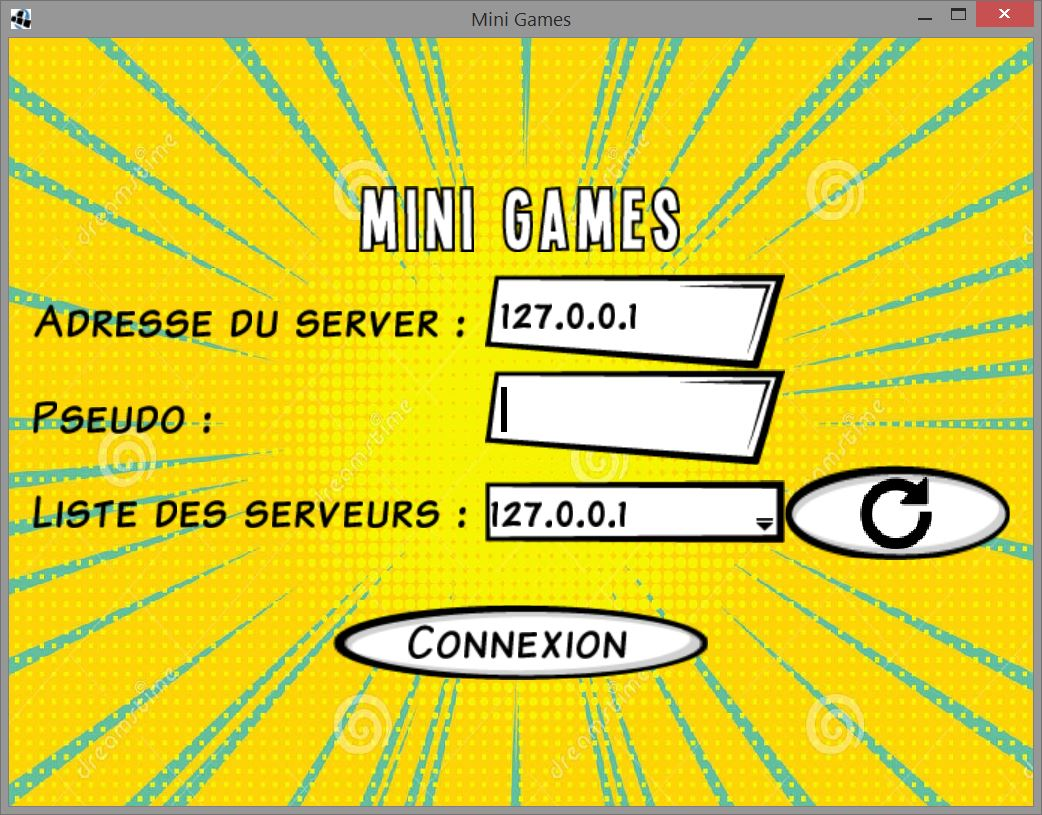
\includegraphics[width=9cm]{loginScreen}
	\caption{Écran de connexion}
\end{figure}

Pour faciliter la connexion au sevreur, un système de recherche des serveurs est disponible. Le recherche se lance
automatiquement au démarrage du programme et peut être relancé à nouveau plus tards en appuyant sur le bouton de rafraichissement.


\chapter{Menu de sélection des minis jeux}
Une fois correctement connecté, vous avez le choix de lancer une partie de morpion ou de bataille navale.
\begin{figure}[H]
	\centering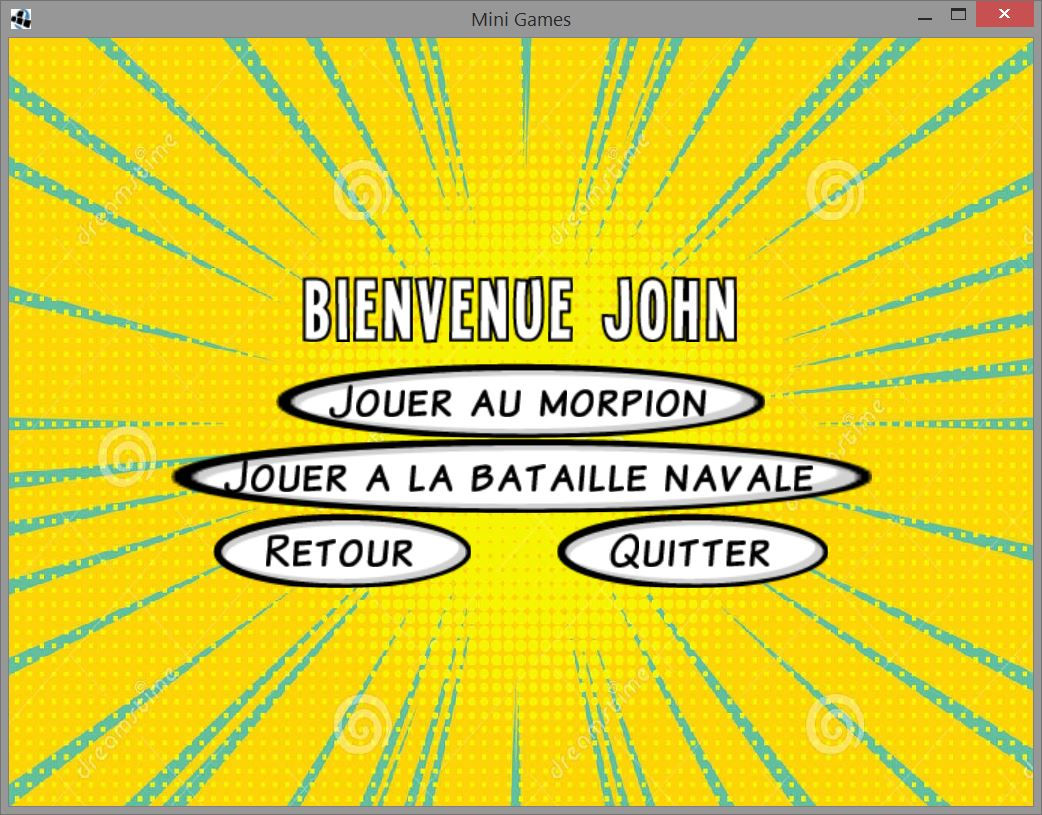
\includegraphics[width=9cm]{MenuJeux}
	\caption{Écran de connexion}
\end{figure}

Avant que la partie en elle-même commence, vous serez au préalable mis en attente le temps que le serveur vous trouve un adversaire. Une fois qu'il vous sera attitré, la partie commencera.

\begin{figure}[H]
	\centering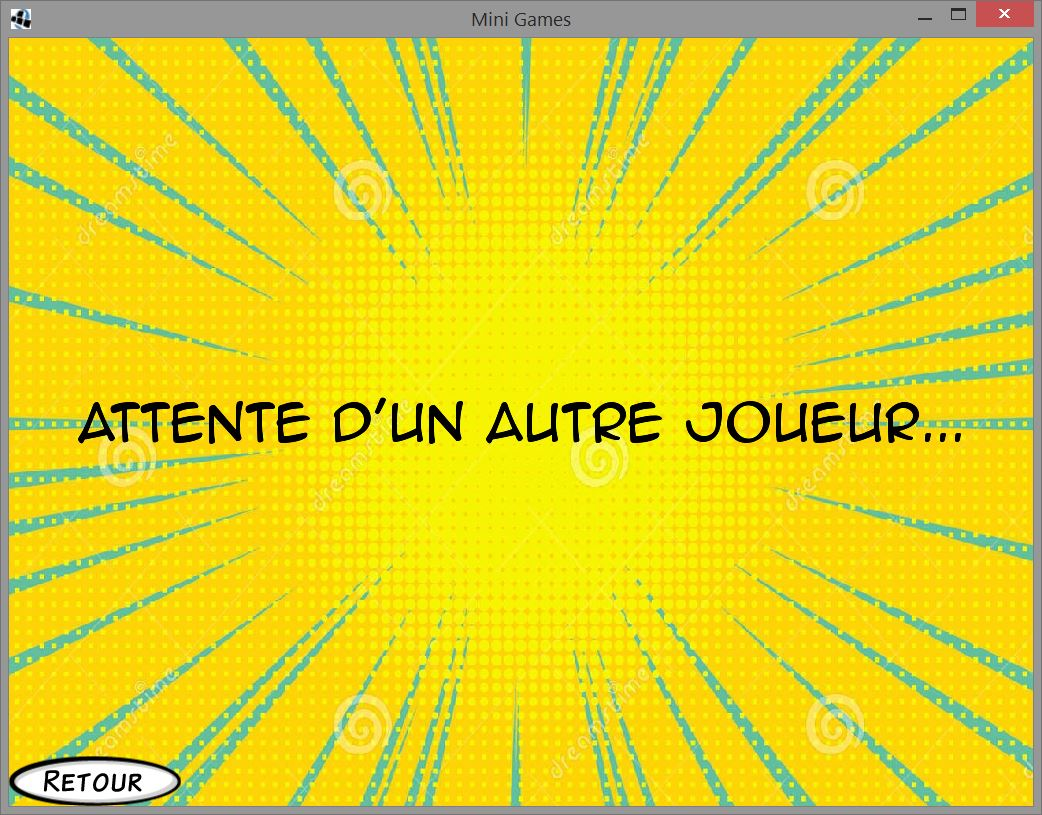
\includegraphics[width=9cm]{morpionwaiting}
	\caption{Écran d'attente}
\end{figure}

\chapter{Morpion}
Le morpion est un jeu qui se joue tour par tour où les joueurs vont placer sur un
plateau de jeu des caractères ('x' ou 'o'). Dès qu'une ligne ou une diagonale est remplie uniquement par un seul caractère,
le joueur ayant rempli cette ligne/diagonale a gagné.

\begin{figure}[H]
	\centering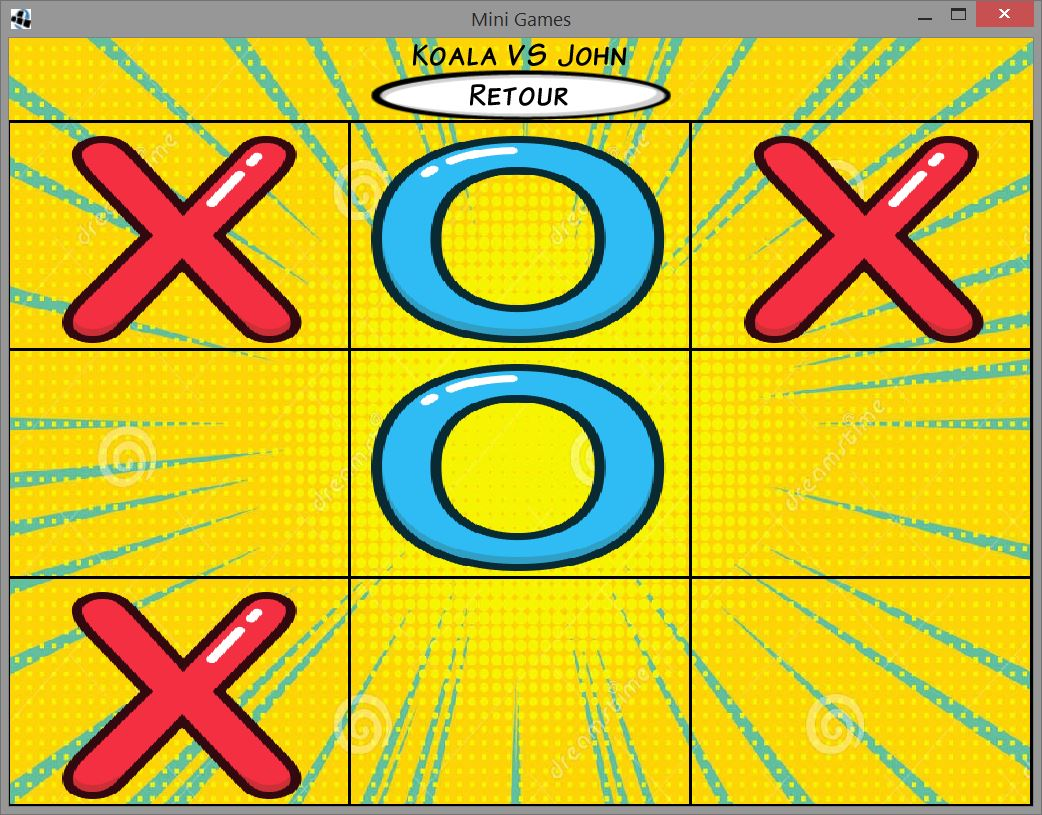
\includegraphics[width=9cm]{morpioningame}
	\caption{Écran de jeu du morpion}
\end{figure}


\chapter{Bataille navale}
Notre jeu de bataille navale, reprend les règles normales du jeu mais avec quelques différences sur le placement et la découverte des bateaux (ennemis ou alliés). Au lieu de pouvoir placer
des bateaux de tailles variables, notre jeu possède des bateaux de taille fixe (une case) 
voir figure \ref{notreBataille}. Il s'agira alors de trouver où son adversaire a caché ses navires avant qu'il ne trouve les nôtres.

\begin{figure}[H]
	\centering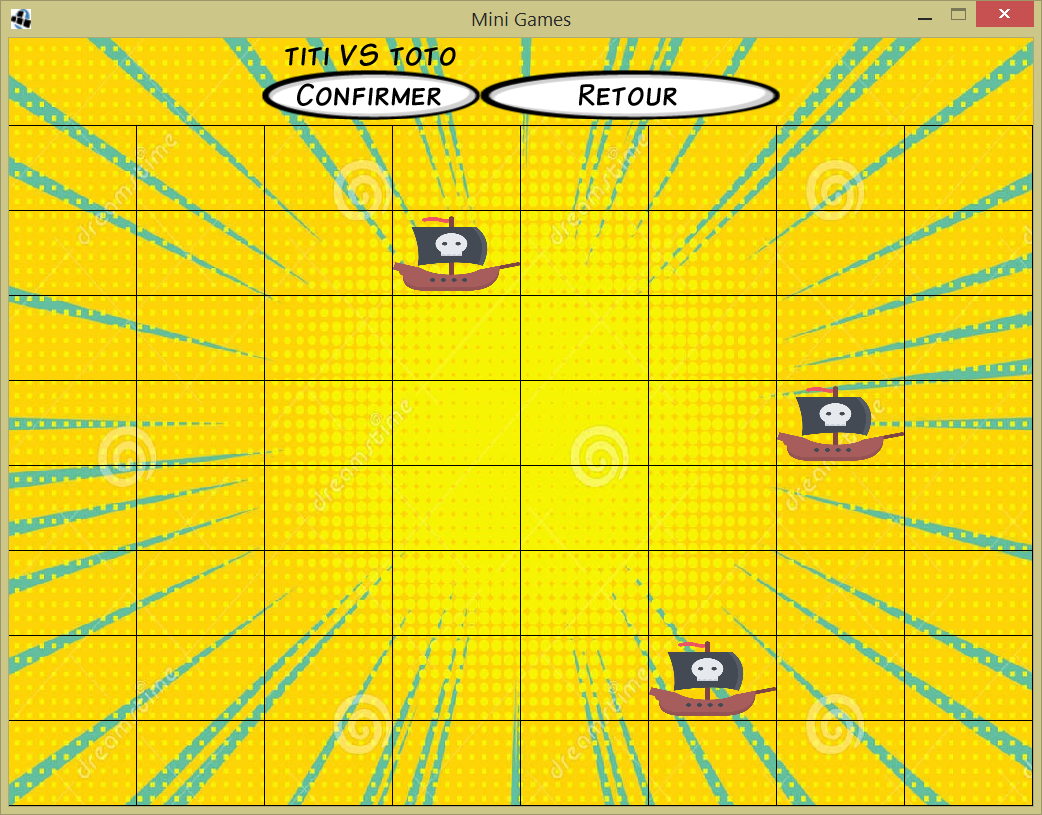
\includegraphics[width=9cm]{notreBataille}
	\caption{Écran de jeu de la bataille navale}
    \label{notreBataille}
\end{figure}

Au début de la partie le joueur doit placer ses bateaux sur le plateau de jeu. Une fois
tous les bateaux placés, le joueur doit cliquer sur le bouton "confirmer" pour valider le placment des bateaux.
Quand les deux adversaires valider leurs placements, la partie peut commencer. Le bouton "confirmer" change alors en un
bouton "inverser" permmettant à l'utilisateur soit d'afficher l'écran de ses bateaux ou l'écran regroupant les endroits où il a tiré. Pour pouvoir tirer le joueur doit impérativement afficher le second écran.


\end{document}
